\section{Numerical evidence and transportation interpretation}\label{sec:numerics}
For Sioux Falls, all reported absolute TSTT accounts use benchmark flows in veh/h and time
units of $0.01$ h; multiply a reported number by $0.01$ to obtain the
hourly vehicle-hour total. This convention applies to the Sioux Falls attribution and error tables.
Anaheim instead uses minutes, as specified separately in Section~\ref{sec:anaheim}.
\subsection{Study design and local mechanism}
The Sioux Falls experiment compares an exactly conservative learned surrogate
with direct fixed-path logit-SUE on eight OD queries. The two evidence
types divide the labour: Figure~\ref{fig:blockcut} illustrates the
classification's query dependence on a network whose queries merge atoms
differently, whereas here all $76$ arcs lie in one compatibility class,
the structural weight condition is the same for every OD, and the
experiment instead measures what boundary differences heterogeneous
realized cost weights produce under equilibrium responses. The OD
differences reported below thus arise from realized responses, weight
dispersion, and integration, not from different compatibility classes.
Each study OD uses ten
fixed paths. We compare zero background (A), frozen background flows (B),
and joint re-equilibration at fixed background demands (C). Setting C loads
all $528$ positive-demand OD pairs but attributes changes only to the eight
study demands, selected as the eight largest published demands --- all
involving node $10$, a local rather than representative comparison.
Appendix~\ref{supp:fields} gives the full settings.

Each study demand moves from $0.2q_{\mathrm{base}}$ to $1.6q_{\mathrm{base}}$
along a straight line ($q_{\mathrm{base}}$: the eight published
demands, $3{,}900$--$4{,}400$ veh/h); the eight-query experiments use this demand
segment unless otherwise stated. The three settings differ only in how
the remaining demands are handled.

The settings also differ in the redistribution directions their
fixed path sets can express: setting A's path-exchange space
$T_{\mathrm{swap}}$ (Appendix~\ref{app:membership}) has dimension
$32$, a proper subspace of the $53$-dimensional circulation space,
while setting C's full-background path set spans the complete space
($53=m-n+1$; Appendix~\ref{supp:networks}). Spanning the circulation
space is a statement about linear directions, not about which signed
responses the logit-SUE Jacobian realizes.

Uniform weights are a compatible control. The inactive-link outcome
$T(F)=F_{1\to2}$ gives zero attribution because that arc lies outside
the setting-A surrogate path union (setting C's path sets cover every
arc). The active-link outcome $T(F)=F_{10\to16}$ gives
$BDx=\mu_{(10,16)}x_{10\to16}$: direction is preserved for that OD, while
circulations can change the scale. TSTT instead weights the response by
heterogeneous marginal social costs and produces interior node imbalance.
Figure~\ref{fig:respfield} shows these three patterns on the same realized
learned response.
\begin{figure}[htbp]
\centering
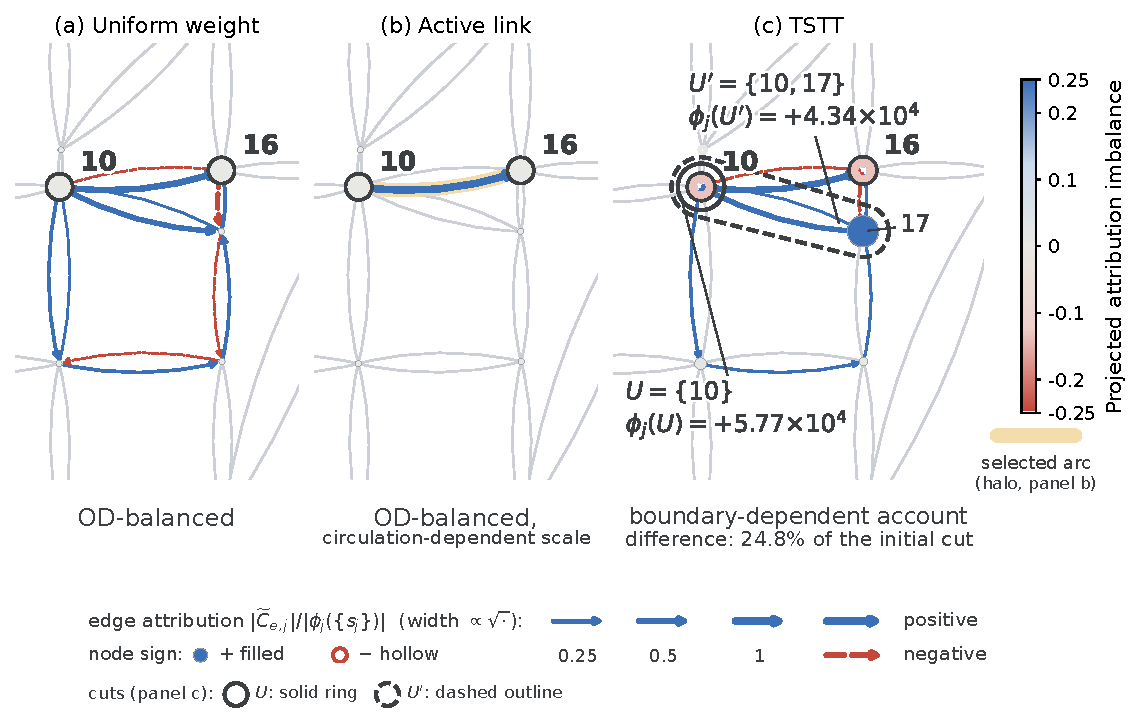
\includegraphics[width=0.84\linewidth]{../figures/fig_resp_field_v100.pdf}
\caption{OD $(10,16)$ endpoint attributions, zero background, learned
seed $0$. (a) Uniform weights give cut consistency. (b) The active-link
outcome balances in the OD direction but has no response-independent scale.
(c) The signed TSTT boundary account decreases by $24.8\%$ when the
boundary expands from $\{10\}$ to $\{10,17\}$.
Widths encode attribution magnitude; node colors show the projected
attribution imbalance $(d_j)_v$ (Eq.~\eqref{eq:endpointd}) divided by
the absolute origin-cut value.}
\label{fig:respfield}
\end{figure}
For the seed-$0$ TSTT account, adding node $17$ to $U=\{10\}$ lowers
$\phi_j(U)$ from $5.77\times10^4$ to $4.34\times10^4$ --- the largest
of the $22$ single-node enlargements, accounting for about $92\%$ of
the unrestricted range, with the direct-SUE counterpart at $24.80\%$
(Section~\ref{subsec:bgsplit}); both displayed regions and their
complements are network-connected.
The free-flow component contributes $84.7\%$ of the node-$17$ imbalance,
the congestion premium $15.3\%$; the ordering reverses at the negative
minima of Section~\ref{subsec:newod}, where the congestion premium
dominates (Table~\ref{tab:ffcong}). All incident links have free-flow time
$2$ except $10\leftrightarrow17$, which has time $8$; exact vehicle balance
gives
\[
[B\operatorname{diag}(t_0)G_j]_{17}
=(8-2)(G_{10\to17,j}-G_{17\to10,j}).
\]
The exchange cancels in vehicle units but not under heterogeneous costs.


\subsection{Background traffic changes the same OD queries}\label{subsec:bgchange}
Table~\ref{tab:cutspreadperod} combines the three demand settings.
With zero background, learned and direct-SUE ranges separate into
four large and four small values. This reflects the realized demand
response rather than fixed OD characteristics; Appendix~\ref{supp:additional}
relates the small ranges to small pointwise imbalance.

Freezing background link flows changes congestion while suppressing
the background route response; letting routes re-equilibrate
produces large ranges for all eight queries --- $(10,16)$ moves from
$26.94\%$ in A to $109.04\%$ in C, the initially near-balanced
$(10,11)$ from $0.0075\%$ to $84.67\%$ (percentages on each
setting's own origin-cut value; per-query absolute denominators in
Appendix~\ref{supp:additional}).

\begin{table}[pos=htbp]
\caption{TSTT cut ranges as percentages of each account's absolute
origin-cut value. A: zero background; B: frozen background flows;
C: background demands fixed, all traffic re-equilibrated. Learned
values are five-seed medians (ranges); all SUE columns are direct
($41$ quadrature points, implicit sensitivities).}
\label{tab:cutspreadperod}
\small
\begin{tabular*}{\tblwidth}{@{\extracolsep{\fill}}lccccc}
\toprule
& \multicolumn{4}{c}{Unrestricted range (\%)} & Connected (\%)\\
\cmidrule(lr){2-5}\cmidrule(lr){6-6}
OD & Learned A & SUE A & SUE B & SUE C & SUE C\\
\midrule
$(17,10)$ & $59.71$ $(58.92$--$61.23)$ & $59.95$ & $56.38$ & $54.77$ & $35.27$ \\
$(10,17)$ & $37.55$ $(37.40$--$37.94)$ & $37.48$ & $43.62$ & $49.11$ & $31.57$ \\
$(16,10)$ & $36.80$ $(36.41$--$38.40)$ & $36.86$ & $39.99$ & $166.26$ & $127.72$ \\
$(10,16)$ & $26.85$ $(26.68$--$27.07)$ & $26.94$ & $34.02$ & $109.04$ & $83.80$ \\
$(15,10)$ & $0.84$ $(0.69$--$1.16)$ & $0.77$ & $21.98$ & $84.05$ & $58.24$ \\
$(10,15)$ & $0.81$ $(0.76$--$0.88)$ & $0.77$ & $18.89$ & $71.88$ & $49.90$ \\
$(10,11)$ & $0.23$ $(0.10$--$0.35)$ & $0.0075$ & $1.17$ & $84.67$ & $51.27$ \\
$(11,10)$ & $0.18$ $(0.03$--$0.27)$ & $0.0073$ & $0.79$ & $81.09$ & $48.98$ \\
\bottomrule
\end{tabular*}
\end{table}
Under re-routing, connected boundaries retain $60.41$--$76.85\%$ of
the unrestricted range (connected ranges $31.57$--$127.72\%$ of the
origin-cut value): connectivity materially narrows the background
envelope but does not restore cut consistency, and the two families
should not be interchanged.


For OD $(17,10)$, the normalized range decreases from
$59.95\%$ in A to $54.77\%$ in C while the absolute range increases
from $17{,}607.8$ to $123{,}202.1$ TSTT units, about sevenfold: a lower percentage need not mean a smaller absolute
difference.

\subsection{Separating the background route response}\label{subsec:bgsplit}
Comparing A, B, and C changes both congestion and sensitivities. To isolate
the background response at the same state, split total flow in setting C
into the sum of the eight study ODs and the other $520$ background ODs.
Then $BJ_j^{\mathrm{study}}=\mu_j$ and $BJ_j^{\mathrm{bg}}=0$.
Weighting both sensitivities, at each quadrature point, by the same
total-flow TSTT gradient gives
\begin{equation}
\widetilde C_j^{\mathrm{tot}}
=\widetilde C_j^{\mathrm{study}}+\widetilde C_j^{\mathrm{bg}}.
\label{eq:bg_attribution}
\end{equation}
At node $15$ for $(10,16)$, the background term contributes
$49{,}103.4$ against the study term's $-973.1$ TSTT units to internal
node divergence. A vehicle-flow circulation can therefore dominate
cost-weighted imbalance (full node breakdown in
Appendix~\ref{supp:additional}, Table~\ref{tab:bgdecomp}).
For a concrete comparison, retain the connected regions $U=\{10\}$
and $U'=\{10,17\}$ from the zero-background illustration --- specified
local regions, not range-attaining ones --- whose complements are also
connected and which separate both queries reported next. With
$g\in\{\mathrm{study},\mathrm{bg},\mathrm{tot}\}$,
\[
\Delta\phi_j^{(g)}
=-\bigl(\mathbf1_{U'}-\mathbf1_U\bigr)^\top B\widetilde C_j^{(g)},
\qquad
\Delta\phi_j^{\mathrm{tot}}=\Delta\phi_j^{\mathrm{study}}+\Delta\phi_j^{\mathrm{bg}}.
\]
At the same equilibrium states, this enlargement changes the $(10,16)$
account by $-3361.1$ ($-1305.0$ study, $-2056.1$ background; $1.23\%$
of $\phi_j(U)$) and the $(10,11)$ account by $-1461.4$ ($-269.9$
study, $-1191.5$ background; $0.72\%$). Thus large extremal ranges
can coexist with small differences at selected sections.
Specified boundary differences add across components, whereas the
absolute ranges satisfy only
$S_j^{\rm tot}\le S_j^{\rm study}+S_j^{\rm bg}$.

\subsection{Boundary-dependent signs across OD queries}\label{subsec:newod}
Six queries away from node $10$ were pre-specified by taking the
shortest and longest free-flow shortest-path ODs within each demand
tercile (demands $200$--$800$ veh/h; path times $2$--$23$;
Appendix~\ref{supp:newod}). Their demands move jointly from $0.2$ to
$1.6$ of published values, with all others fixed; all $528$ ODs
re-equilibrate under the setting-C protocol.

Table~\ref{tab:newod} reports the result: all six system contributions
$C_j$ are positive, but for the three queries with the longest
free-flow shortest-path times the minimum--maximum ranges straddle
zero in both the unrestricted and the connected family. OD $(1,19)$,
for instance, has an origin-cut account of $1{,}771.6$ TSTT units
while its connected-family accounts range from $-13{,}502$ to
$24{,}260$: the boundary choice can change the sign of the reported
account, not merely its magnitude. Negative accounts occur in
$17.8\%$, $2.5\%$, and $7.3\%$ of the $14{,}477$, $15{,}191$, and
$16{,}943$ enumerated connected boundaries of $(1,19)$, $(1,15)$, and
$(7,12)$; no connected boundary of the three sign-consistent queries
is negative. These are shares of the enumerated family, not the odds
of an analyst drawing such a boundary. For the three crossing queries
the system contribution exceeds the origin-cut account by factors of
twelve to twenty-eight; for the three sign-consistent queries the two
agree within a factor of $1.6$, so a boundary account is not a
rescaled system contribution even when the two are close. OD
$(6,8)$'s unrestricted range of $99.75\%$ (connected $65.22\%$) shows
that the sign is set by the extrema themselves, not by the size of
the normalized range.

\begin{table}[pos=htbp]
\caption{System contributions and spatial ranges for six prespecified queries,
setting C (TSTT units). Connected: all admissible connected regions;
screenline: the geometric family constructed independently of attribution
values. All $C_j$ are positive. Origin-cut accounts, negative shares, and
neighbourhood ranges are retained in Appendix~\ref{supp:newodaccuracy}.}
\label{tab:newod}
\small
\begin{tabular*}{\tblwidth}{@{\extracolsep{\fill}}lrrr}
\toprule
OD & $C_j$ & Connected [min, max] & Screenline [min, max]\\
\midrule
$(7,18)$ & $672.9$ & $[634{,}\ 710]$ & $[642{,}\ 702]$ \\
$(1,19)$ & $50{,}097.7$ & $[-13{,}502{,}\ 24{,}260]$ & $[-2{,}767{,}\ 22{,}124]$ \\
$(4,5)$ & $2{,}826.0$ & $[2{,}396{,}\ 3{,}452]$ & $[2{,}652{,}\ 3{,}176]$ \\
$(1,15)$ & $77{,}403.2$ & $[-8{,}286{,}\ 40{,}540]$ & $[511{,}\ 36{,}621]$ \\
$(6,8)$ & $73{,}964.9$ & $[35{,}307{,}\ 66{,}695]$ & $[45{,}230{,}\ 65{,}286]$ \\
$(7,12)$ & $117{,}482.3$ & $[-17{,}616{,}\ 60{,}029]$ & $[-2{,}967{,}\ 57{,}780]$ \\
\bottomrule
\end{tabular*}
\end{table}

Why one connected boundary attains a negative account is visible in
the attribution columns: by Eq.~\eqref{eq:cutextrema}, sign crossing
in the unrestricted family is decided by the interior positive
divergence against the origin-cut
account, which it exceeds by factors of about $5.8$ to $12$. For
$(1,19)$, the connected
minimum $-13{,}501.6$ is attained by a $13$-node connected region
containing the origin. The free-flow-time neighbourhood at radius $16$
also contains $13$ nodes, yet its account is $+10{,}756.0$.
By Eq.~\eqref{eq:cutgap}, their respective net interior divergences
are approximately $+15{,}273.1$ and $-8{,}984.4$ TSTT units:
the account depends on the spatial distribution of weighted demand
responses within the region, rather than its node count alone
(node sets in Appendix~\ref{supp:newodaccuracy}).

At the boundary itself, entering links contribute $-21{,}368.8$ and
leaving links $+7{,}867.3$ to the twenty-six-link signed sum,
dominated by large \emph{positive} attributions on
\emph{entering} links; Figure~\ref{fig:negmech} maps the region and
each link's signed contribution in the appendix. For
the joint six-query demand change, $\phi_j(U^-)$ is OD $j$'s
contribution to the change in the signed boundary cost sum $H_{U^-}$
(Eq.~\eqref{eq:hboundary}); the total change of $H_{U^-}$ sums all six
varying ODs' contributions, and $C_j=50{,}097.7>0$.
Different regions define different functions $H_U$, so opposite signs
are compatible with integrated gradients. The classification addresses
when their summaries can serve as one transferable OD account;
otherwise Eq.~\eqref{eq:cutgap} explains their differences.

The BPR marginal cost $g_e'=t_{0,e}+0.75t_{0,e}(F_e/c_e)^4$
splits the weights into free-flow and congestion-premium parts.
Combining this with the study/background response split at each of
the same equilibrium states gives, at the fixed reported $U_-$,
\[
\phi_j(U_-)=\phi_j^{\mathrm{ff,study}}+\phi_j^{\mathrm{ff,bg}}
+\phi_j^{\mathrm{cong,study}}+\phi_j^{\mathrm{cong,bg}},
\qquad
\phi_j^{a,b}=-\Delta q_j\int_0^1\mathbf1_{U_-}^{\top}
BD_\lambda^aJ_j^b(\lambda)\,d\lambda.
\]
Table~\ref{tab:ffcong} locates the negative account differently across
queries: the study congestion term dominates for $(1,19)$, both
congestion terms are negative for $(1,15)$, and background congestion
dominates for $(7,12)$. The combined free-flow part stays positive
at all three boundaries. This is an additive explanation at the same
states and fixed boundaries, not a causal effect of removing
background traffic or congestion. The interior-divergence split in
Appendix~\ref{supp:newodaccuracy} concerns a different sum and cannot
be substituted for this boundary decomposition.
\begin{table}[pos=htbp]
\caption{Four parts of the same boundary account at the reported
$U_-$ (setting C, six-query protocol; TSTT units; identical $41$-point
states, responses, and boundaries as Table~\ref{tab:newod}). Study
includes all six query ODs; background includes the other $522$.
Columns cross free-flow/congestion weights with study/background
responses. Entries are rounded independently.}
\label{tab:ffcong}
\small
\begin{tabular*}{\tblwidth}{@{\extracolsep{\fill}}lrrrrr}
\toprule
OD & ff, study & ff, background & cong, study & cong, background & Total\\
\midrule
$(1,19)$ & $-361.3$ & $+759.0$ & $-17{,}357.9$ & $+3{,}458.6$ & $-13{,}501.6$ \\
$(1,15)$ & $+1{,}541.8$ & $+333.8$ & $-6{,}537.4$ & $-3{,}624.2$ & $-8{,}286.0$ \\
$(7,12)$ & $+3{,}897.0$ & $-1{,}311.1$ & $+125.5$ & $-20{,}327.6$ & $-17{,}616.2$ \\
\bottomrule
\end{tabular*}
\end{table}

\begin{figure}[pos=tb]
\centering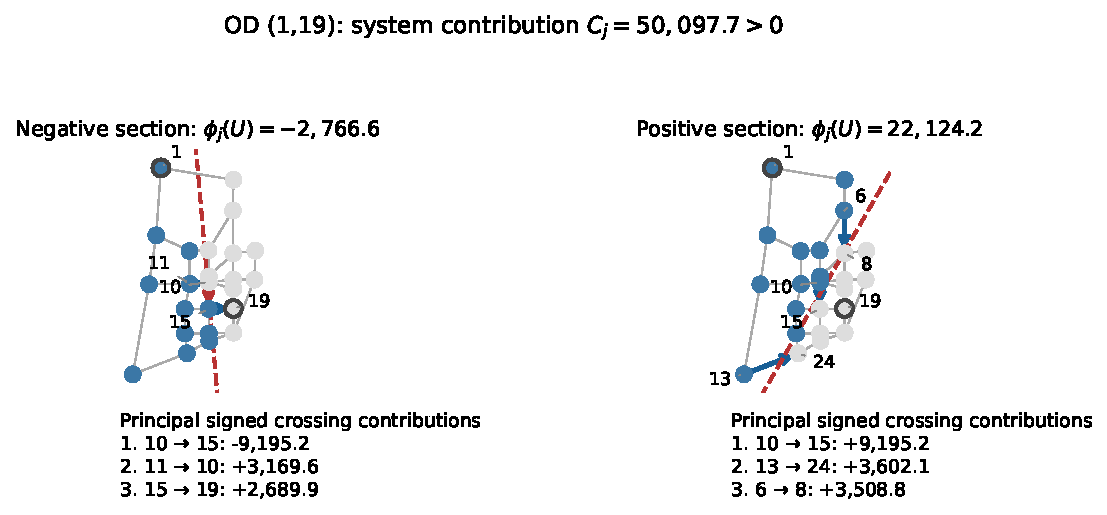
\includegraphics[width=0.99\linewidth]{../figures/fig_screenlines_v103.pdf}
\caption{Two straight screenlines for OD $(1,19)$, setting C. Blue nodes
belong to $U$; grey nodes are outside; dashed lines separate the two
sides. Node $1$ is inside and node $19$ outside in both panels. The two
accounts have opposite signs while the network-wide contribution is
positive. The lines are the minimum and maximum of the prespecified
geometric family; the complete irregular connected minimum and its
crossing-link decomposition appear in Figure~\ref{fig:negmech}.}
\label{fig:screenlines}\end{figure}


The enumerated extrema establish existence within the admissible
family; the prescribed boundaries separate sign from magnitude. All
tested origin-centred hop-distance and free-flow-time neighbourhood
accounts remain positive, yet within those families the largest account
is $8.9$, $9.0$, and $3.4$ times the smallest for $(1,19)$, $(1,15)$,
and $(7,12)$ (Appendix~\ref{supp:newodaccuracy}): sign stability does not mean that
simple, network-distance-defined boundaries give comparable magnitudes.
Straight screenlines sharpen the picture. Projecting the public node
coordinates onto $36$ pre-fixed directions ($5^\circ$ apart, both sides
of each line kept, positions midway between adjacent node projections,
connectedness and deduplication as in the connected family; no
attribution value enters the construction;
Appendix~\ref{supp:newodaccuracy}) yields $23$--$152$ distinct
straight-line boundaries per query. On these, $(1,19)$ and $(7,12)$
again attain negative accounts (minima $-2{,}767$ and $-2{,}967$ TSTT
units, on $2$ of $152$ and $10$ of $148$ boundaries), shallower than
the enumerated minima, while the remaining four queries in the screenline family stay
positive with magnitudes spanning up to a factor of $72$ for $(1,15)$
($511$--$36{,}621$). Practical straight-line sections therefore do not
inherit the sign safety of the neighbourhood families, nor do their
positive accounts agree in magnitude. Appendix~\ref{supp:newodaccuracy} reports the path-set, dispersion,
single-OD, and narrow-band checks. The separable TSTT structure gives a
particularly direct interpretation when only one demand changes:
\begin{equation}
\widetilde C_{e,j}=g_e(F_e^1)-g_e(F_e^0),\qquad g_e(F_e)=F_et_e(F_e).
\label{eq:edgeidentity}
\end{equation}
Indeed $dF_e/d\lambda=\Delta q_j\partial_jf_e$ along that path, so the
fundamental theorem of calculus applies link by link, including background
rerouting. Consequently $\phi_j(U)=H_U(f(q^1))-H_U(f(q^0))$: a negative
single-OD boundary account is an actual decrease in that signed boundary
cost sum. This identity also checks the numerical edge attribution directly.

